\documentclass{standalone}
\usepackage{tikz}
\usetikzlibrary[arrows,decorations.pathmorphing,backgrounds,positioning,matrix,fit,calc]

\makeatletter
\newcommand{\gettikzx}[2]{%
  \tikz@scan@one@point\pgfutil@firstofone#1\relax
  \edef#2{\the\pgf@x}%
}
% Get y-coordinate of node
\newcommand{\gettikzy}[2]{%
  \tikz@scan@one@point\pgfutil@firstofone#1\relax
  \edef#2{\the\pgf@y}%
}
% Get x- and y- coordinate of node
\newcommand{\gettikzxy}[3]{%
  \tikz@scan@one@point\pgfutil@firstofone#1\relax
  \edef#2{\the\pgf@x}%
  \edef#3{\the\pgf@y}%
}
%
\pgfdeclareshape{document}{
  \inheritsavedanchors[from=rectangle] % this is nearly a rectangle
  \inheritanchorborder[from=rectangle]
  \inheritanchor[from=rectangle]{center}
  \inheritanchor[from=rectangle]{north}
  \inheritanchor[from=rectangle]{south}
  \inheritanchor[from=rectangle]{west}
  \inheritanchor[from=rectangle]{east}
  % ... and possibly more
  \backgroundpath{% this is new
    % store lower right in xa/ya and upper right in xb/yb
    \southwest \pgf@xa=\pgf@x \pgf@ya=\pgf@y
    \northeast \pgf@xb=\pgf@x \pgf@yb=\pgf@y
    % compute corner of ‘‘flipped page’’
    \pgf@xc=\pgf@xb \advance\pgf@xc by-10pt % this should be a parameter
    \pgf@yc=\pgf@yb \advance\pgf@yc by-10pt
    % construct main path
    \pgfpathmoveto{\pgfpoint{\pgf@xa}{\pgf@ya}}
    \pgfpathlineto{\pgfpoint{\pgf@xa}{\pgf@yb}}
    \pgfpathlineto{\pgfpoint{\pgf@xc}{\pgf@yb}}
    \pgfpathlineto{\pgfpoint{\pgf@xb}{\pgf@yc}}
    \pgfpathlineto{\pgfpoint{\pgf@xb}{\pgf@ya}}
    \pgfpathclose
    % add little corner
    \pgfpathmoveto{\pgfpoint{\pgf@xc}{\pgf@yb}}
    \pgfpathlineto{\pgfpoint{\pgf@xc}{\pgf@yc}}
    \pgfpathlineto{\pgfpoint{\pgf@xb}{\pgf@yc}}
    \pgfpathlineto{\pgfpoint{\pgf@xc}{\pgf@yc}}
  }
}
\makeatother
%
% all other packages and stuff you need for the picture
%
\begin{document}
% ===== System Modelling =====

\newsavebox{\modelling}% Comment needs to be here, otherwise space is added!
\savebox{\modelling}{% Comment needs to be here, otherwise space is added!
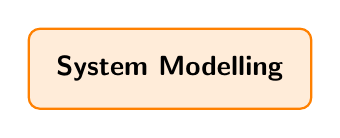
\begin{tikzpicture}[font=\sffamily]
  \node[rectangle,rounded corners,thick,draw=orange,fill=orange!15,align=center,inner sep =10pt] 
       {\textbf{System Modelling}};
\end{tikzpicture}% Comment needs to be here, otherwise space is added!
}% Comment needs to be here, otherwise space is added!
%
%
% ===== APPLICATION MODELS =====
%
% -- Draw acyclic graph
\newsavebox{\acyclic}% Comment needs to be here, otherwise space is added!%
\savebox{\acyclic}{% Comment needs to be here, otherwise space is added!
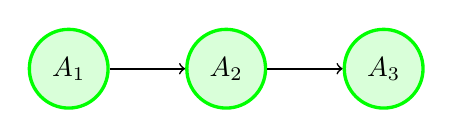
\begin{tikzpicture}[
font=\sffamily,
signal/.style={rectangle,draw=black,fill=gray!0,thick,minimum size=3mm},
actor/.style={circle,draw=green,fill=green!15,very thick, inner
  sep=0pt,minimum size=10mm, node distance=15mm},
application/.style={rectangle,draw=black,fill=black!10,ultra thick},
operation/.style={rectangle,rounded corners,draw=black,fill=black!10,ultra thick},
dot/.style={circle,fill=black,minimum size=5pt,inner sep=0},
arrow/.style={->,semithick}
]
\node[actor] (a) {$A_1$};
\node[actor] (b) [xshift = 2cm] {$A_2$};
\node[actor] (c) [xshift = 4cm] {$A_3$};
\draw[arrow] (a.east) node [above right] {\small } -- (b.west) node [above left] {\small };
\draw[arrow] (b.east) node [above right] {\small } -- (c.west) node [above left] {\small };

\end{tikzpicture}% Comment needs to be here, otherwise space is added!
}% Comment needs to be here, otherwise space is added!
%
% -- Draw cyclic graph
\newsavebox{\cyclic}% Comment needs to be here, otherwise space is added!
\savebox{\cyclic}{% Comment needs to be here, otherwise space is added!
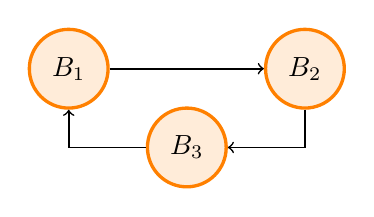
\begin{tikzpicture}[
font=\sffamily,
signal/.style={rectangle,draw=black,fill=gray!0,thick,minimum size=3mm},
actor/.style={circle,draw=orange,fill=orange!15,very thick, inner
  sep=0pt,minimum size=10mm, node distance=15mm},
application/.style={rectangle,draw=black,fill=black!10,ultra thick},
operation/.style={rectangle,rounded corners,draw=black,fill=black!10,ultra thick},
dot/.style={circle,fill=black,minimum size=5pt,inner sep=0},
arrow/.style={->,semithick}
]

\node[actor] (b1) {$B_1$};
\node[actor] (b2) [xshift=3cm] {$B_2$};
\node[actor] (b3) [yshift=-1cm, xshift=1.5cm] {$B_3$};
\draw[arrow] (b1.east) node [above right] {\small } -- (b2.west) node [above left] {\small };
\draw[arrow] (b2) node [above right] {\small } |- (b3) node [above left] {\small };
\draw[arrow] (b3) node [above right] {\small } -| (b1) node [above left] {\small };
\end{tikzpicture}% Comment needs to be here, otherwise space is added!
}% Comment needs to be here, otherwise space is added!
%
\newsavebox{\application}% Comment needs to be here, otherwise space is added!
\savebox{\application}{% Comment needs to be here, otherwise space is added!
\begin{tikzpicture}[
font=\sffamily
]
\node (acyclic) {\usebox{\acyclic}}; 
\node (cyclic) [yshift = -2cm] {\usebox{\cyclic}}; 
\end{tikzpicture}% Comment needs to be here, otherwise space is added!
}% Comment needs to be here, otherwise space is added!
%
% ===== DESIGN CONSTRAINTS =====
%
\newsavebox{\constraints}% Comment needs to be here, otherwise space is added!
\savebox{\constraints}{% Comment needs to be here, otherwise space is added!
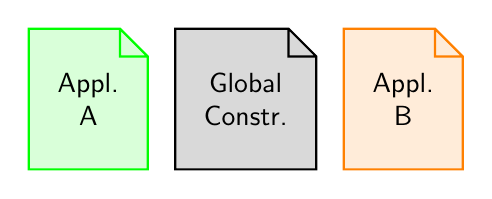
\begin{tikzpicture}[
font=\sffamily,
doc/.style={document,thick,inner sep=10pt,minimum height=5em, minimum width=3em,align=center} 
]
  \node[doc,draw=green,fill=green!15]   (a) at (-2,0) {Appl. \\ A} ;
  \node[doc,draw=black,fill=black!15]   (a) at (0,0) {Global \\ Constr.} ;
  \node[doc,draw=orange,fill=orange!15] (b) at (2,0){Appl. \\ B};
%  \node at (0,\north) [above] {Design Constraints};
\end{tikzpicture}% Comment needs to be here, otherwise space is added!
}% Comment needs to be here, otherwise space is added!
%
%
% ===== PLATFORM MODEL =====
%
\newsavebox{\platform}% Comment needs to be here, otherwise space is added!
\savebox{\platform}{% Comment needs to be here, otherwise space is added!
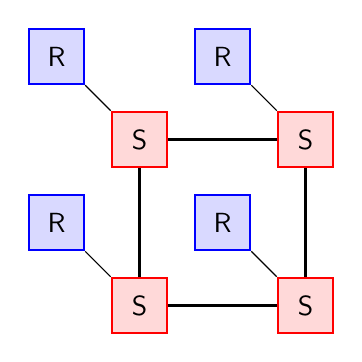
\begin{tikzpicture}[
font=\sffamily,
resource/.style={rectangle,draw=blue,fill=blue!15,thick,inner sep=3pt,minimum height=2em,minimum width=2em},
switch/.style={rectangle,draw=red,fill=red!15,thick,inner sep=3pt,minimum height=2em,minimum width=2em},
channel/.style={thick}
]

% Set size of NoC
\def\rows{2}
\def\columns{2}

\pgfmathtruncatemacro\m{int(\columns-1)}
\pgfmathtruncatemacro\n{int(\rows-1)}
\foreach \x in {0,...,\m}{
  \foreach \y in {0,...,\n} {
    \node [switch]  [xshift=6*\x em] [yshift=-6*\y em] (s\x\y) {S};
    \node [resource] [xshift=6*\x em - 3em] [yshift=-6*\y em+3em] (r\x\y) {R};
    \draw (s\x\y) to (r\x\y);
  }
}

% Draw channels in y-direction
\foreach \x in {0,...,\m}{
   \pgfmathtruncatemacro\k{\n-1};
   \foreach \y in {0,...,\k}{
     \pgfmathtruncatemacro\incy{int(\y + 1)}
     \draw [channel] (s\x\incy) to ({s\x\y});
  }
}

% Draw channels in x-direction

\foreach \y in {0,...,\n}{
   \pgfmathtruncatemacro\l{\m-1};
   \foreach \x in {0,...,\l}{
      \pgfmathtruncatemacro\incx{int(\x+1)};
      \draw [channel] (s\x\y) to ({s\incx\y});
   }
}
\end{tikzpicture}% Comment needs to be here, otherwise space is added!
}% Comment needs to be here, otherwise space is added!
%
% ===== Performance Metrics  =====

\newsavebox{\metrics}% Comment needs to be here, otherwise space is added!
\savebox{\metrics}{% Comment needs to be here, otherwise space is added!
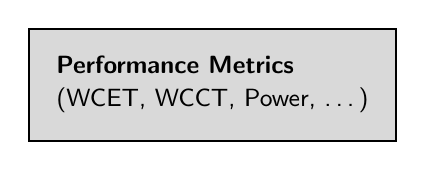
\begin{tikzpicture}[font=\sffamily]
  \node[rectangle,thick,draw=black,fill=black!15,align=left,inner sep =10pt] 
       {\textbf{\small Performance Metrics}\\
        \small (WCET, WCCT, Power, \dots)};
\end{tikzpicture}% Comment needs to be here, otherwise space is added!
}% Comment needs to be here, otherwise space is added!
 
% ===== Design Space Exploration =====

\newsavebox{\dse}% Comment needs to be here, otherwise space is added!
\savebox{\dse}{% Comment needs to be here, otherwise space is added!
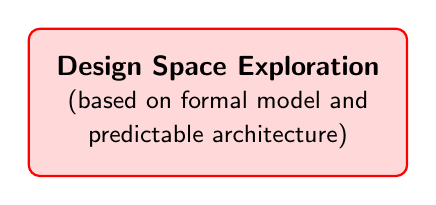
\begin{tikzpicture}[font=\sffamily]
  \node[rectangle,rounded corners,thick,draw=red,fill=red!15,align=center,inner sep =10pt] 
       {\textbf{Design Space Exploration}\\
        \small (based on formal model and\\
        \small predictable architecture)};
\end{tikzpicture}% Comment needs to be here, otherwise space is added!
}% Comment needs to be here, otherwise space is added!
%
% ===== MAPPING =====
%
\newsavebox{\mapping}% Comment needs to be here, otherwise space is added!
\savebox{\mapping}{% Comment needs to be here, otherwise space is added!
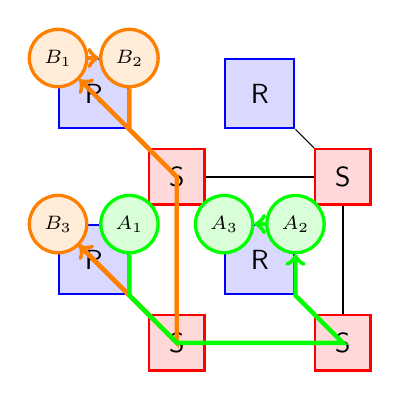
\begin{tikzpicture}[
font=\sffamily,
resource/.style={rectangle,draw=blue,fill=blue!15,thick,inner sep=3pt,minimum height=2.5em,minimum width=2.5em},
switch/.style={rectangle,draw=red,fill=red!15,thick,inner sep=3pt,minimum height=2em,minimum width=2em},
channel/.style={thick},
actorA/.style={circle,draw=green,fill=green!15,very thick, minimum size=3mm},
actorB/.style={circle,draw=orange,fill=orange!15,very thick, minimum size=3mm},
connectionA/.style={->, ultra thick, draw=green},
connectionB/.style={->, ultra thick, draw=orange},
]

% Set size of NoC
\def\rows{2}
\def\columns{2}

\pgfmathtruncatemacro\m{int(\columns-1)}
\pgfmathtruncatemacro\n{int(\rows-1)}
\foreach \x in {0,...,\m}{
  \foreach \y in {0,...,\n} {
    \node [switch]  [xshift=6*\x em] [yshift=-6*\y em] (s\x\y) {S};
    \node [resource] [xshift=6*\x em - 3em] [yshift=-6*\y em+3em] (r\x\y) {R};
    \draw (s\x\y) to (r\x\y);
  }
}

% Draw channels in y-direction
\foreach \x in {0,...,\m}{
   \pgfmathtruncatemacro\k{\n-1};
   \foreach \y in {0,...,\k}{
     \pgfmathtruncatemacro\incy{int(\y + 1)}
     \draw [channel] (s\x\incy) to ({s\x\y});
  }
}

% Draw channels in x-direction

\foreach \y in {0,...,\n}{
   \pgfmathtruncatemacro\l{\m-1};
   \foreach \x in {0,...,\l}{
      \pgfmathtruncatemacro\incx{int(\x+1)};
      \draw [channel] (s\x\y) to ({s\incx\y});
   }
}

% Node 0,0: B1, B2
\node[actorB] (b1) at (r00.north west) {\scriptsize $B_1$};
\node[actorB] (b2) at (r00.north east) {\scriptsize $B_2$};

% Node 0,1: A1, B3
\node[actorB] (b3) at (r01.north west) {\scriptsize $B_3$};
\node[actorA] (a1) at (r01.north east) {\scriptsize $A_1$};

% Node 1,0: A3
% --- Empty

% Node 1,1: A2
\node[actorA] (a2) at (r11.north east) {\scriptsize $A_2$};
\node[actorA] (a3) at (r11.north west) {\scriptsize $A_3$};

\draw[connectionB] (b1) to (b2);
\draw[connectionB] (b2.south) -- (r00.south east) -- (s00.center) -- (s01.center) -- (b3);
\draw[connectionB] (b3) -- (s01) -- (s00) -- (r00.south east) -- (b1);

\draw[connectionA] (a1) -- (r01.south east) -- (s01.center) -- (s11.center) -- (r11.south east) -- (a2);
\draw[connectionA] (a2) -- (a3);
\end{tikzpicture}% Comment needs to be here, otherwise space is added!
}% Comment needs to be here, otherwise space is added!
%
% ===== SYNTHESIS =====
%
\newsavebox{\synthesis}% Comment needs to be here, otherwise space is added!
\savebox{\synthesis}{% Comment needs to be here, otherwise space is added!
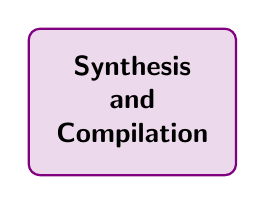
\begin{tikzpicture}[font=\sffamily]
  \node[rectangle,rounded corners,thick,draw=violet,fill=violet!15,align=center,inner sep =10pt] 
       {\textbf{Synthesis}\\ 
        \textbf{and}\\
        \textbf{Compilation}};
\end{tikzpicture}% Comment needs to be here, otherwise space is added!
}% Comment needs to be here, otherwise space is added!
%
% ===== CHIP =====
%
\newsavebox{\chip}% Comment needs to be here, otherwise space is added!
\savebox{\chip}{% Comment needs to be here, otherwise space is added!
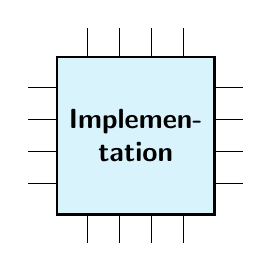
\begin{tikzpicture}[
font=\sffamily,
chip/.style={rectangle,draw=black,fill=cyan!15,thick,inner sep=3pt,minimum height=2cm,minimum width=2cm},
connector/.style={}
]

% Draw Chip
\node [chip,align=center] (chip) {\textbf{Implemen-}\\\textbf{tation}};

% Get coordinates (N,E,S,W) and sidelength
\gettikzy{(chip.north)}{\north};
\gettikzy{(chip.south)}{\south};
\gettikzx{(chip.east)}{\east};
\gettikzx{(chip.west)}{\west};
\pgfmathsetmacro\length{\east-\west};


% Draw connectors: North and South

\foreach \x in {1,...,4}{
  \pgfmathsetmacro\newx{\west+\x/5*\length};
  \pgfmathsetmacro\newy{\north+10};
  \coordinate (p1) at (\newx pt, \north);
  \coordinate (p2) at (\newx pt, \newy pt);
  \draw [connector,draw=black] (p1) to (p2);

  \pgfmathsetmacro\newy{\south-10};
  \coordinate (p1) at (\newx pt, \south);
  \coordinate (p2) at (\newx pt, \newy pt);
  \draw [connector,draw=black] (p1) to (p2);
}

% Draw connectors: East and West

\foreach \x in {1,...,4}{
  \pgfmathsetmacro\newy{\south+\x/5*\length};
  \pgfmathsetmacro\newx{\east+10};
  \coordinate (p1) at (\east, \newy pt);
  \coordinate (p2) at (\newx pt, \newy pt);
  \draw [connector,draw=black] (p1) to (p2);

  \pgfmathsetmacro\newx{\west-10};
  \coordinate (p1) at (\west, \newy pt);
  \coordinate (p2) at (\newx pt, \newy pt);
  \draw [connector,draw=black] (p1) to (p2);
}


\end{tikzpicture}% Comment needs to be here, otherwise space is added!
}% Comment needs to be here, otherwise space is added!
%

\begin{tikzpicture}[
font=\sffamily,
arrow/.style={->, draw=red!70, ultra thick},
]

% -- System Modelling
  \node (modelling)         at (-6,7)  {\usebox{\modelling}};


% -- Application
\node  (application) at (-6,4) {\scalebox{0.9}{\usebox{\application}}};
  \node[rectangle,text width=4.5cm,anchor=north, inner sep=0pt] (text) at (application.south) [yshift=-5pt] { \small
    \textbf{Analyzable Application Models}
    {\begin{itemize}
        \item formal base (MoCs)
        \item executable
    \end{itemize}}
};


% -- Design Constraints
  \node (constraints) at (0, 4) {\scalebox{0.9}{\usebox{\constraints}}};
  \node[rectangle,text width=3.5cm,anchor=south, inner sep=0pt] (text) at  (constraints.north) [yshift=5pt] {\small
    \textbf{Design Constraints}
    {\begin{itemize}
        \item real-time
        \item power and energy
        \item \dots
    \end{itemize}}
};

% -- Platform
  \node  (platform)    at (5.5,5.5)  {\scalebox{1.0}{\usebox{\platform}}};
  \node[rectangle,text width=4.2cm,anchor=north, inner sep=0pt] (text) at  (platform.south) [xshift=20pt,yshift=-5pt] {\small
    \textbf{Platform Architecture}
    {\begin{itemize}
        \item multiprocessor
        \item predictable performance
    \end{itemize}}
};

% -- System Modelling
\draw [arrow] (modelling.south) to (application.north);

% -- Design Space Exploration 
\node (dse)         at (0,0.5)  {\usebox{\dse}};

\draw [arrow] ([yshift=15pt]application.south east) to (dse.north west);
\draw [arrow] (constraints.south) to (dse.north);
\draw [arrow] ([yshift=-10pt]platform.south west) to (dse.north east);

% -- Metrics
\node (metrics)         at (6,0.5)  {\usebox{\metrics}};

\draw [arrow] (metrics.west) to (dse.east);
% -- Mapping
  \node (mapping)     at (-5.5,-3){\usebox{\mapping}};
  \node[rectangle,anchor=south, inner sep=0pt] at (mapping.north) [yshift =5pt]{\small
    \textbf{Mapping and Schedules}
};

\draw [arrow] (dse.south west) to ($ (mapping.north east) + (-0.5,-1)$);

% -- Synthesis
  \node  (synthesis)   at (-0.5,-3) {\usebox{\synthesis}};

\draw [arrow] (mapping.east) to (synthesis.west);

% -- Implementation
  \node  (chip)        at (3.5,-3) {\usebox{\chip}};
  \node[rectangle,text width=4.2cm,anchor=west, inner sep=0pt] at  (chip.east) [xshift=3pt] {\small
    \textbf{Implementation}
    {\begin{itemize}
        \item Customized hardware
        \item Efficient software
    \end{itemize}}
};

\draw [arrow] (synthesis.east) to (chip.west);
\end{tikzpicture}
\end{document} 